\chapter{Laser scanning~\cite{scanning-handbook}}
Všechny obrázky v~této kapitole pocházejí ze~zdroje~\cite{scanning-handbook}, pokud není uvedeno jinak.

Jako Laser scanning se~označuje technologie využívající rychle se pohybující laserový paprsek. Mezi tradfiční techniky pohybu paprsku spadají akusticko-optické skenery, hranolové skenery a galvanometrové skenery~\cite{mems-review}.

\section{Akusticko-optické skenery}
Akusticko-optické~(AO) skenery se využívají, se nejlépe hodí do systémů s rozlišením\footnote{Rozlišení laserových skenerů je počet všech různých pozic, do kterých je skener schopen nasměrovat paprsek.} přibližně 1000 bodů.
Další charakteristikou AO skenerů je možnost přenést paprsek na libovolný bod v časovém úseku řádově 10~\mu.

Existuje mnoho systému využívajících AO skenery, možná nejzajímavější jsou laserové tiskárny, které naplno využívají schopnosti AO skenerů.

Princip AO spočívá pouze ve změně indexu lomu materiálu optiky, když ním prochází akustická vlna. Tato změna indexu lomu způsobí změnu směru paprsku.

\section{Hranolové skenery}
Hranolové skenery se~vyznačují rotujícím hranolem se~zrcadlivými stranami (dále \uv{zrcátky}). Při rotaci hranolu se~mění úhel dopadu laserového paprsku na~zrcátko, a~díky tomu se~mění směr odraženého paprsku, viz. obrázek \ref{fig:polygon-scanner}. \fxnote{adiky carka?}

\begin{figure}[H]
  \centering
  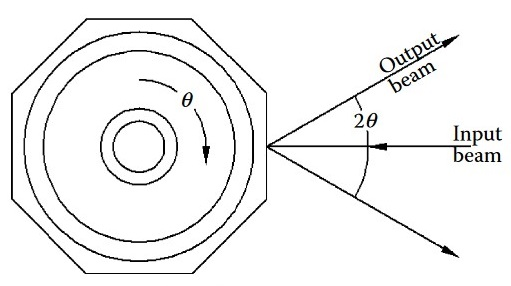
\includegraphics[width=0.5\textwidth]{img/polygon-scanner.jpg}
  \caption{\label{fig:polygon-scanner} mechanika polygonových skenerů}
\end{figure}

% \begin{figure}[!htb]
%   \centering
%   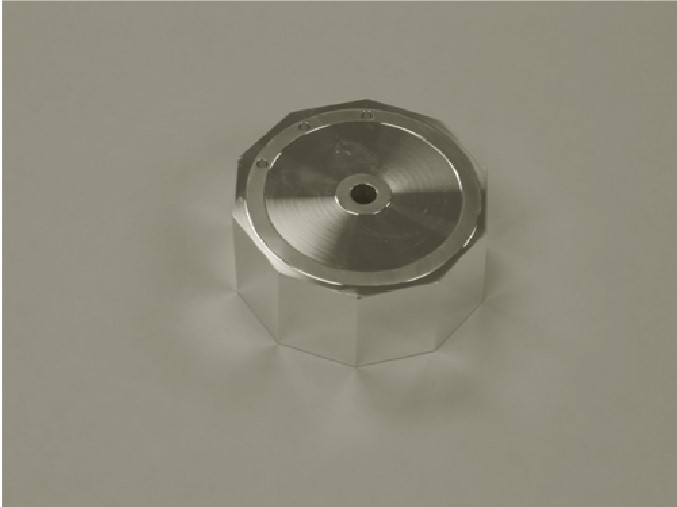
\includegraphics[width=0.5\textwidth]{img/polygon-prismatic-mirror.jpg}
%   \caption{\label{fig:polygon-prismatic-mirror} hranolové zrcátko polygonového skeneru}
% \end{figure}

% \begin{figure}[!htb]
%   \centering
%   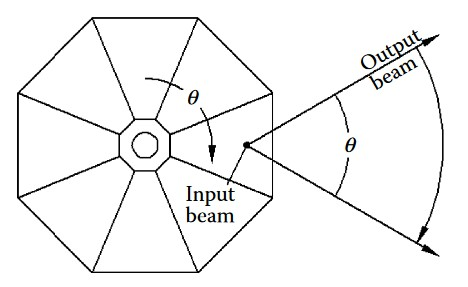
\includegraphics[width=0.5\textwidth]{img/polygon-pyramidal-mirror.jpg}
%   \caption{\label{fig:polygon-pyramidal-mirror} pyramidové zrcátko polygonového skeneru}
% \end{figure}
%

S jedním hranolem by~hranolové skenery byly schopny směřovat paprsek pouze v~jedné rovině - při projekci by~bylo možné vykreslit maximálně čáru. Tuto limitaci lze kompenzovat přidáním melého rozdílu ve~směřování každé strany hranolu, viz. obrázek \ref{fig:polygon-angular-variation}. S~touto úpravou každá strana hranolu "vykreslí" jednu, svoji, přímku lehce posunutou vůči přímkách ostatních stran. Hranol s~n-úhelníkovou podstavou je~schopen vykreslit n~přímek.
Další možností je~kombinovat původní pravidelný hranol s~galvanometrem (popsáno níže), kdy galvanometr nastaví jednu souřadnici paprsku a~hranol na~této souřadnici vykreslí přímku.

Tento typ skeneru se~využívá hlavně pro senzory skenující na~přímce (např. skenery čárových kódů~\cite{history-of-barcode-scanning}), nebo při rastrovém procházení plochy (například 3D skenování, nebo promítání ploch, viz. Obrázek \ref{fig:harddrive-projector-youtube}).

\begin{figure}[!htb]
  \centering
  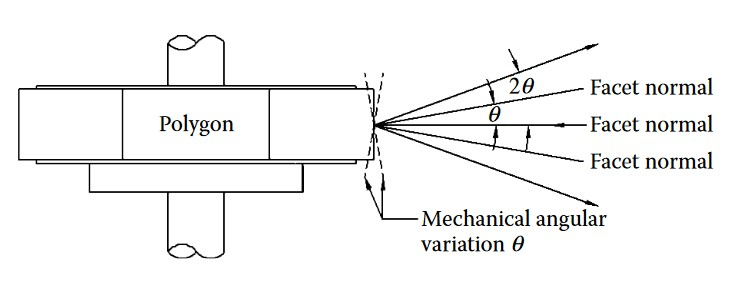
\includegraphics[width=0.8\textwidth]{img/polygon-angular-variation.jpg}
  \caption{\label{fig:polygon-angular-variation} úhlová rozdílnost zrcátek polygonového skeneru a~paprsky od~nich odražené}
\end{figure}


\begin{figure}[!htb]
  \centering
  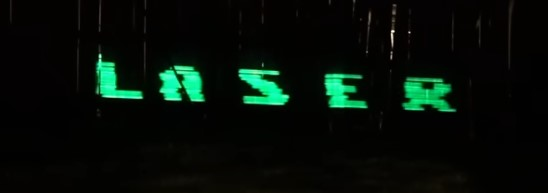
\includegraphics[width=0.5\textwidth]{img/harddrive-projection.jpg}
  \caption{\label{fig:harddrive-projection} příklad projekce laserového projektoru s~polygonovým skenerem; zdroj~\cite{harddrive-projector-youtube}}
\end{figure}

\section{Galvanometrové skenery}
V galvanometrových skenerech paprsek odráží zrcátka/o připevněná/o na~páru galvanometrů.

\subsection{Galvanometr}
Slovem galvanometr se~označuje přístroj úrčený k~detekci nebo měření velice malého elektrického proudu~\cite{galvo-definition}. Galvanometry při měření využívají interakce magnetického pole trvalého magnetu a~cívky protéké proudem. Tato interakce vychýlí ručičku ukazující na~stupnici, nebo zrcátko odrážející paprsek, který dopadá na~stupnici.~\cite{wiki-galvo}

Galvanometry se~dají rozdělit na~galvanometry bez zpětné vazby (open-loop) a~se zpětnou vazbou. K~těm bývají připojeny ovládací obvody, které z~galvanometrů získávají informace o~jejich pohybu a~podle nich regulují signál posílaný do~galvanometrů.~\cite{wiki-galvo}

Dále se~dělí dle pohyblivé součástky. V~galvanometru je~buď trvalý magnet pevně ukotven a~cívka pohyblivá (moving coil), nebo naopak (moving magnet). % https://prirucka.ujc.cas.cz/?id=151#nadpis3

Dnes se~v~kontextu laserových skenerů prakticky vždy používají galvanometry s~pohyblivým magnetem a~se~zpětnou vazbou. Ta~je zajištěna čtením z~variabilního kondenzátoru umístěného v~galvanometru.

\begin{figure}[!htb]
  \centering
  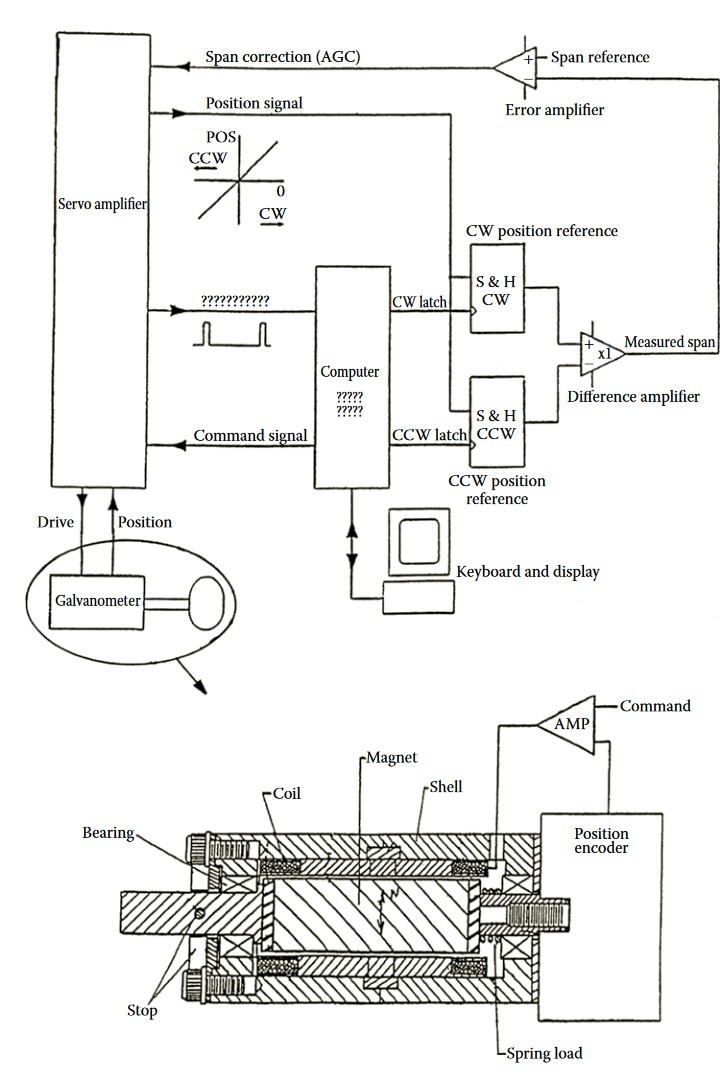
\includegraphics[width=1\textwidth]{img/galvanometer-detail.jpg}
  \caption{\label{fig:galvanometer-detail} zapojení a~vnitřní konstrukce galvanometrů}
\end{figure}

\subsection{Konstrukce galvanometrových skenerů\label{sec:galvo-scanner-construction}}
Jeden galvanometrový skener vždy ovládá jednu osu pohybu paprsku, buď X~nebo Y.

Narozdíl od~hranolových skenerů je~s galvanometrovým skenerem možné zastavit obě osy pohybu - vykreslovat na~sebe kolmé čáry.

\begin{figure}[!htb]
  \centering
  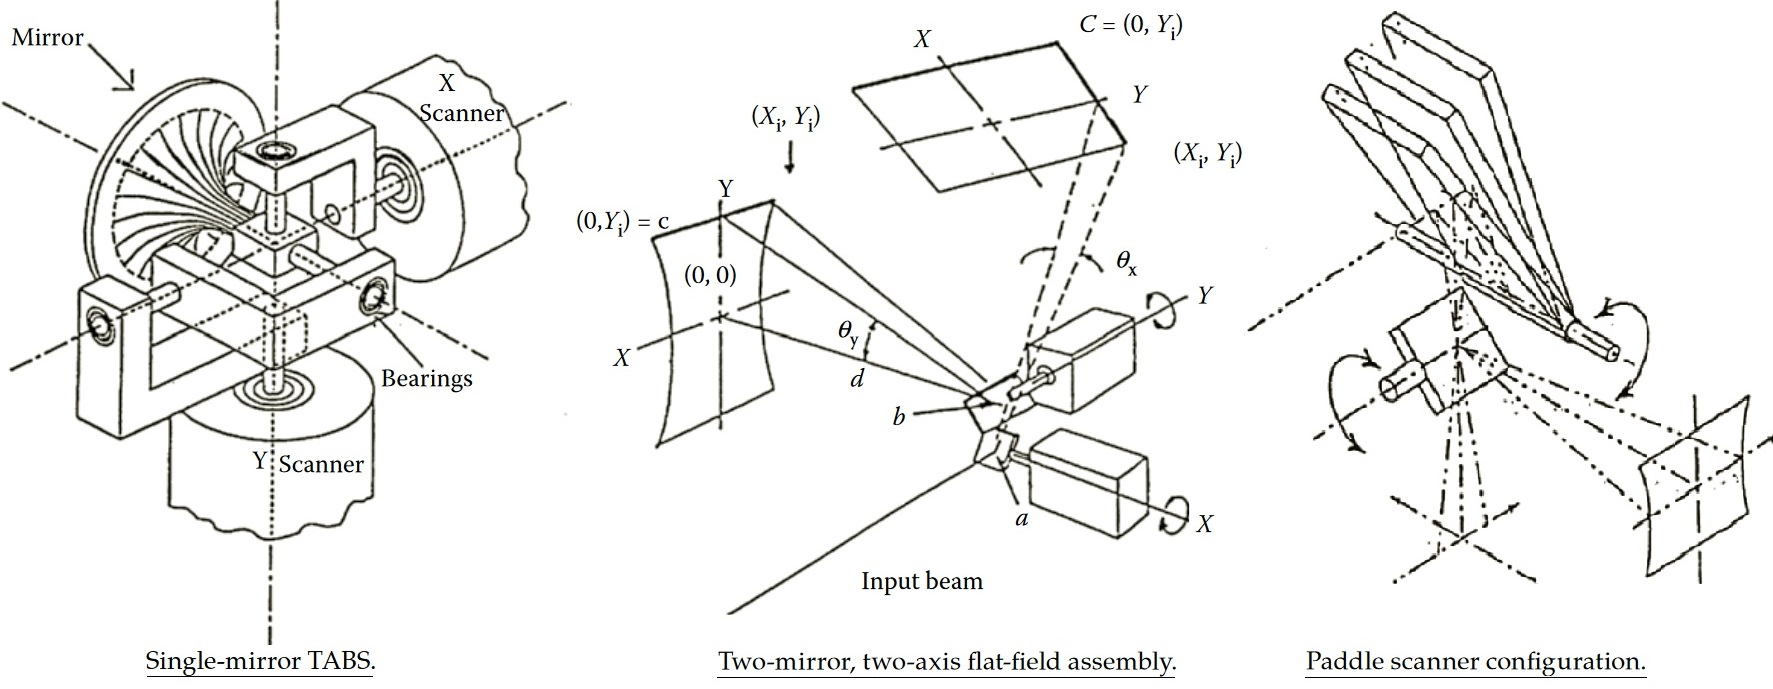
\includegraphics[width=1\textwidth]{img/scanner-constructions.jpg}
  \caption{\label{fig:scanner-constructions} různé konstrukce galvanometrových skenerů}
\end{figure}
